\documentclass[12pt, compress]{beamer}

\usetheme{m}

\usepackage{booktabs}
\usepackage[scale=2]{ccicons}
\usepackage{minted}
\usepackage{tikz}
\usetikzlibrary{intersections}
\usepackage{pgfplots}
\usepackage{standalone}
\usepackage{array}
\usepackage[percent]{overpic}

% Math packages
\usepackage{amsthm}
\usepackage{amssymb}
\usepackage{mathtools}
\usepackage{amsfonts}
\usepackage{amsmath}
\usepackage{kbordermatrix}
\usepackage{blkarray}

% Bibliography
\usepackage{natbib}
\bibpunct{[}{]}{,}{a}{}{;}


% For presentation mode
%\usepackage{pgfpages}
%\setbeameroption{show notes}
%\setbeameroption{show notes on second screen=right}

% Numbered sections in table of contents
\setbeamertemplate{section in toc}[sections numbered]

\usemintedstyle{trac}

\title{Attenuation-based Light Field Displays}
\subtitle{Bachelor Thesis}
\date{June 3, 2016}
\author{Adrian W\"alchli}
\institute{Institut f\"ur Informatik und angewandte Mathematik}

\begin{document}

\setlength{\leftmargini}{0pt}
\setlength{\fboxsep}{0pt}%

\maketitle

\begin{frame}[fragile]
	\frametitle{Outline}
	\tableofcontents
\end{frame}

\section{Motivation}

\begin{frame}[fragile]
	\frametitle{Existing 3D Displays}
	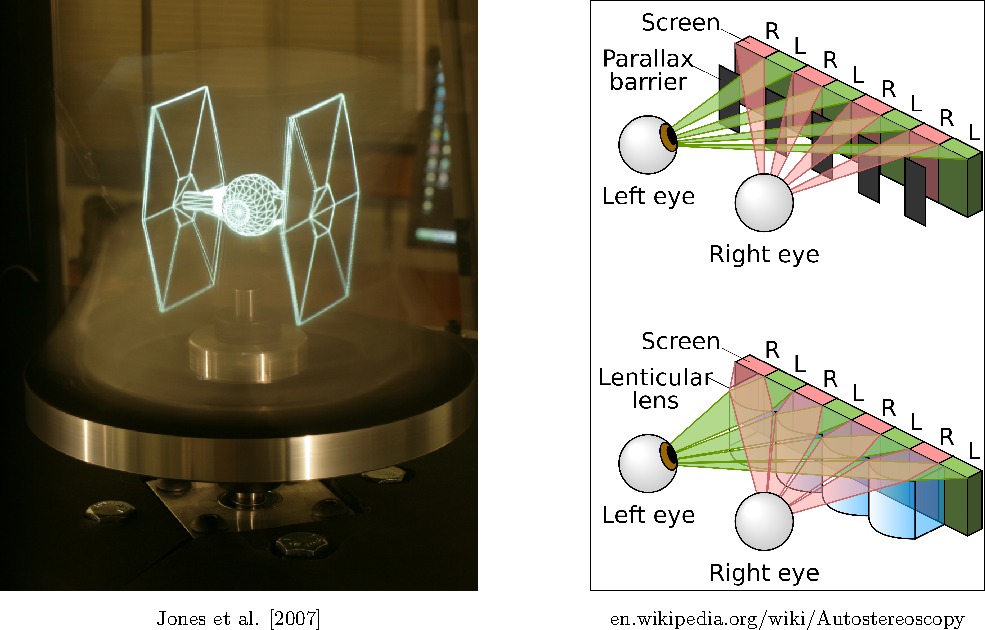
\includegraphics[height = 7cm]{figures/overview_displays/existing_3d_displays.pdf}
\end{frame}

\section{Introduction to Light Fields}

\begin{frame}[fragile]
	\frametitle{The Plenoptic Function}
	
	\begin{columns}[onlytextwidth]
		\column{0.6\textwidth}
			\begin{itemize}[<alert@+>]
				\item Measures light in the world
				\item Position, viewing direction
				\item Time, Wavelength
				\item $P(x, y, z, \theta, \phi, t, \lambda)$
				\item 7D
			\end{itemize}
		\column{0.4\textwidth}
			\vspace{-5cm}
			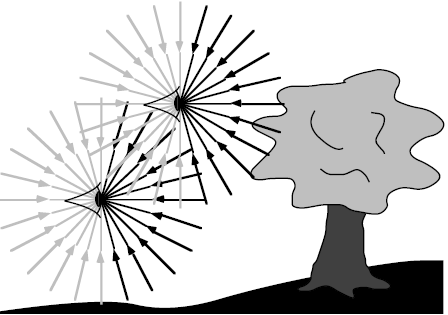
\includegraphics[width = 4cm]{images/plenoptic.png}
	\end{columns}
	
\end{frame}

\begin{frame}[fragile]
	\frametitle{The 4D Light Field}
	
	\begin{itemize}[<alert@+>]
		\item Reduce dimensions of $P$
		\item $L(u, v, s, t)$
		\item Defined by two planes
	\end{itemize}
	\begin{center}
		\visible<3>{\documentclass{standalone}
\usepackage{tikz}

\begin{document}
	
	\begin{tikzpicture}[scale = 0.4]
	
		\filldraw[draw = black, fill = white] (0, 0) -- (5, -2) -- (5, 5) -- (0, 7) -- cycle;
		\filldraw[draw = black, fill = white] (9, 3) -- (14, 1) -- (14, 8) -- (9, 10) -- cycle;
		
		\draw[<-] (-3, 4) -- (1, 4);
		\draw (5, 4) -- (11, 4);
		\draw (14, 4) -- (17, 4);
		
		\node [left] at (-3, 4) {$L(u, v, s, t)$};
		
		
		\draw[fill] (1, 4) circle [radius = 0.1];
		\draw[fill] (11, 4) circle [radius = 0.1];
		
		\node[below right] at (1, 4) {$(u, v)$};
		\node[below right] at (11, 4) {$(s, t)$};
	
	\end{tikzpicture}
	
\end{document}}
	\end{center}
\end{frame}

\begin{frame}[fragile]
	\frametitle{Light Field Acquisition}
	
	\begin{itemize}[<alert@+>]
		\item Camera array
		\item Gantry
		\item Plenoptic camera
	\end{itemize}
	
	\begin{center}
		\visible<1,2,3>{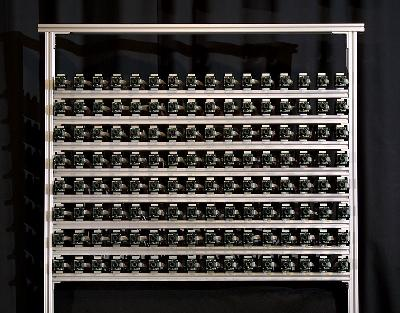
\includegraphics[height = 3.1cm]{images/stanford_camera_array_2.jpg}}
		\hspace{0.2cm}
		\visible<2, 3>{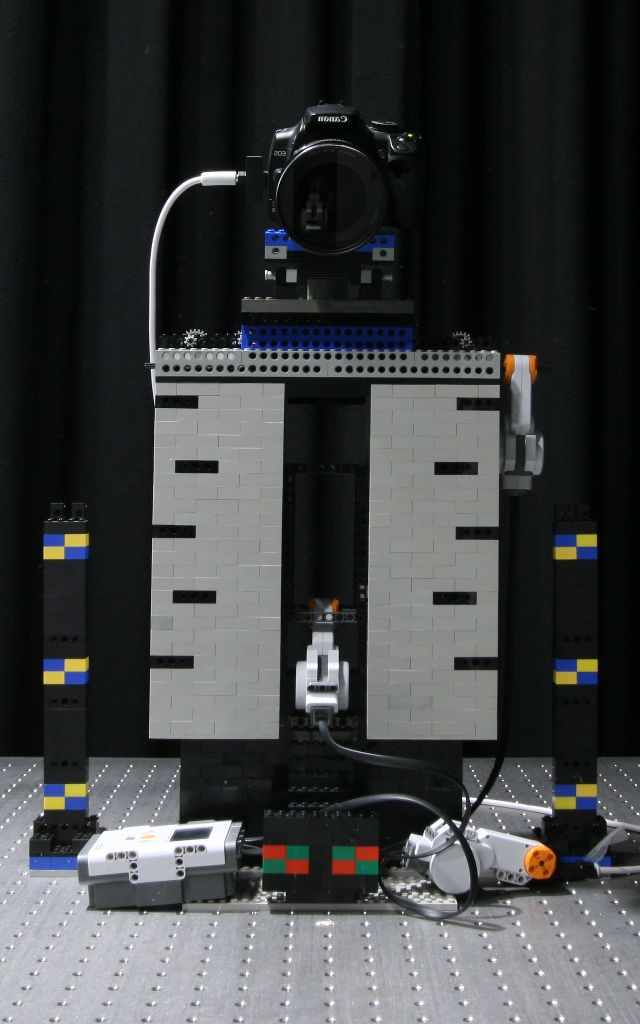
\includegraphics[height = 3.1cm]{images/lego_camera_gantry}}
		\hspace{0.2cm}
		\visible<3>{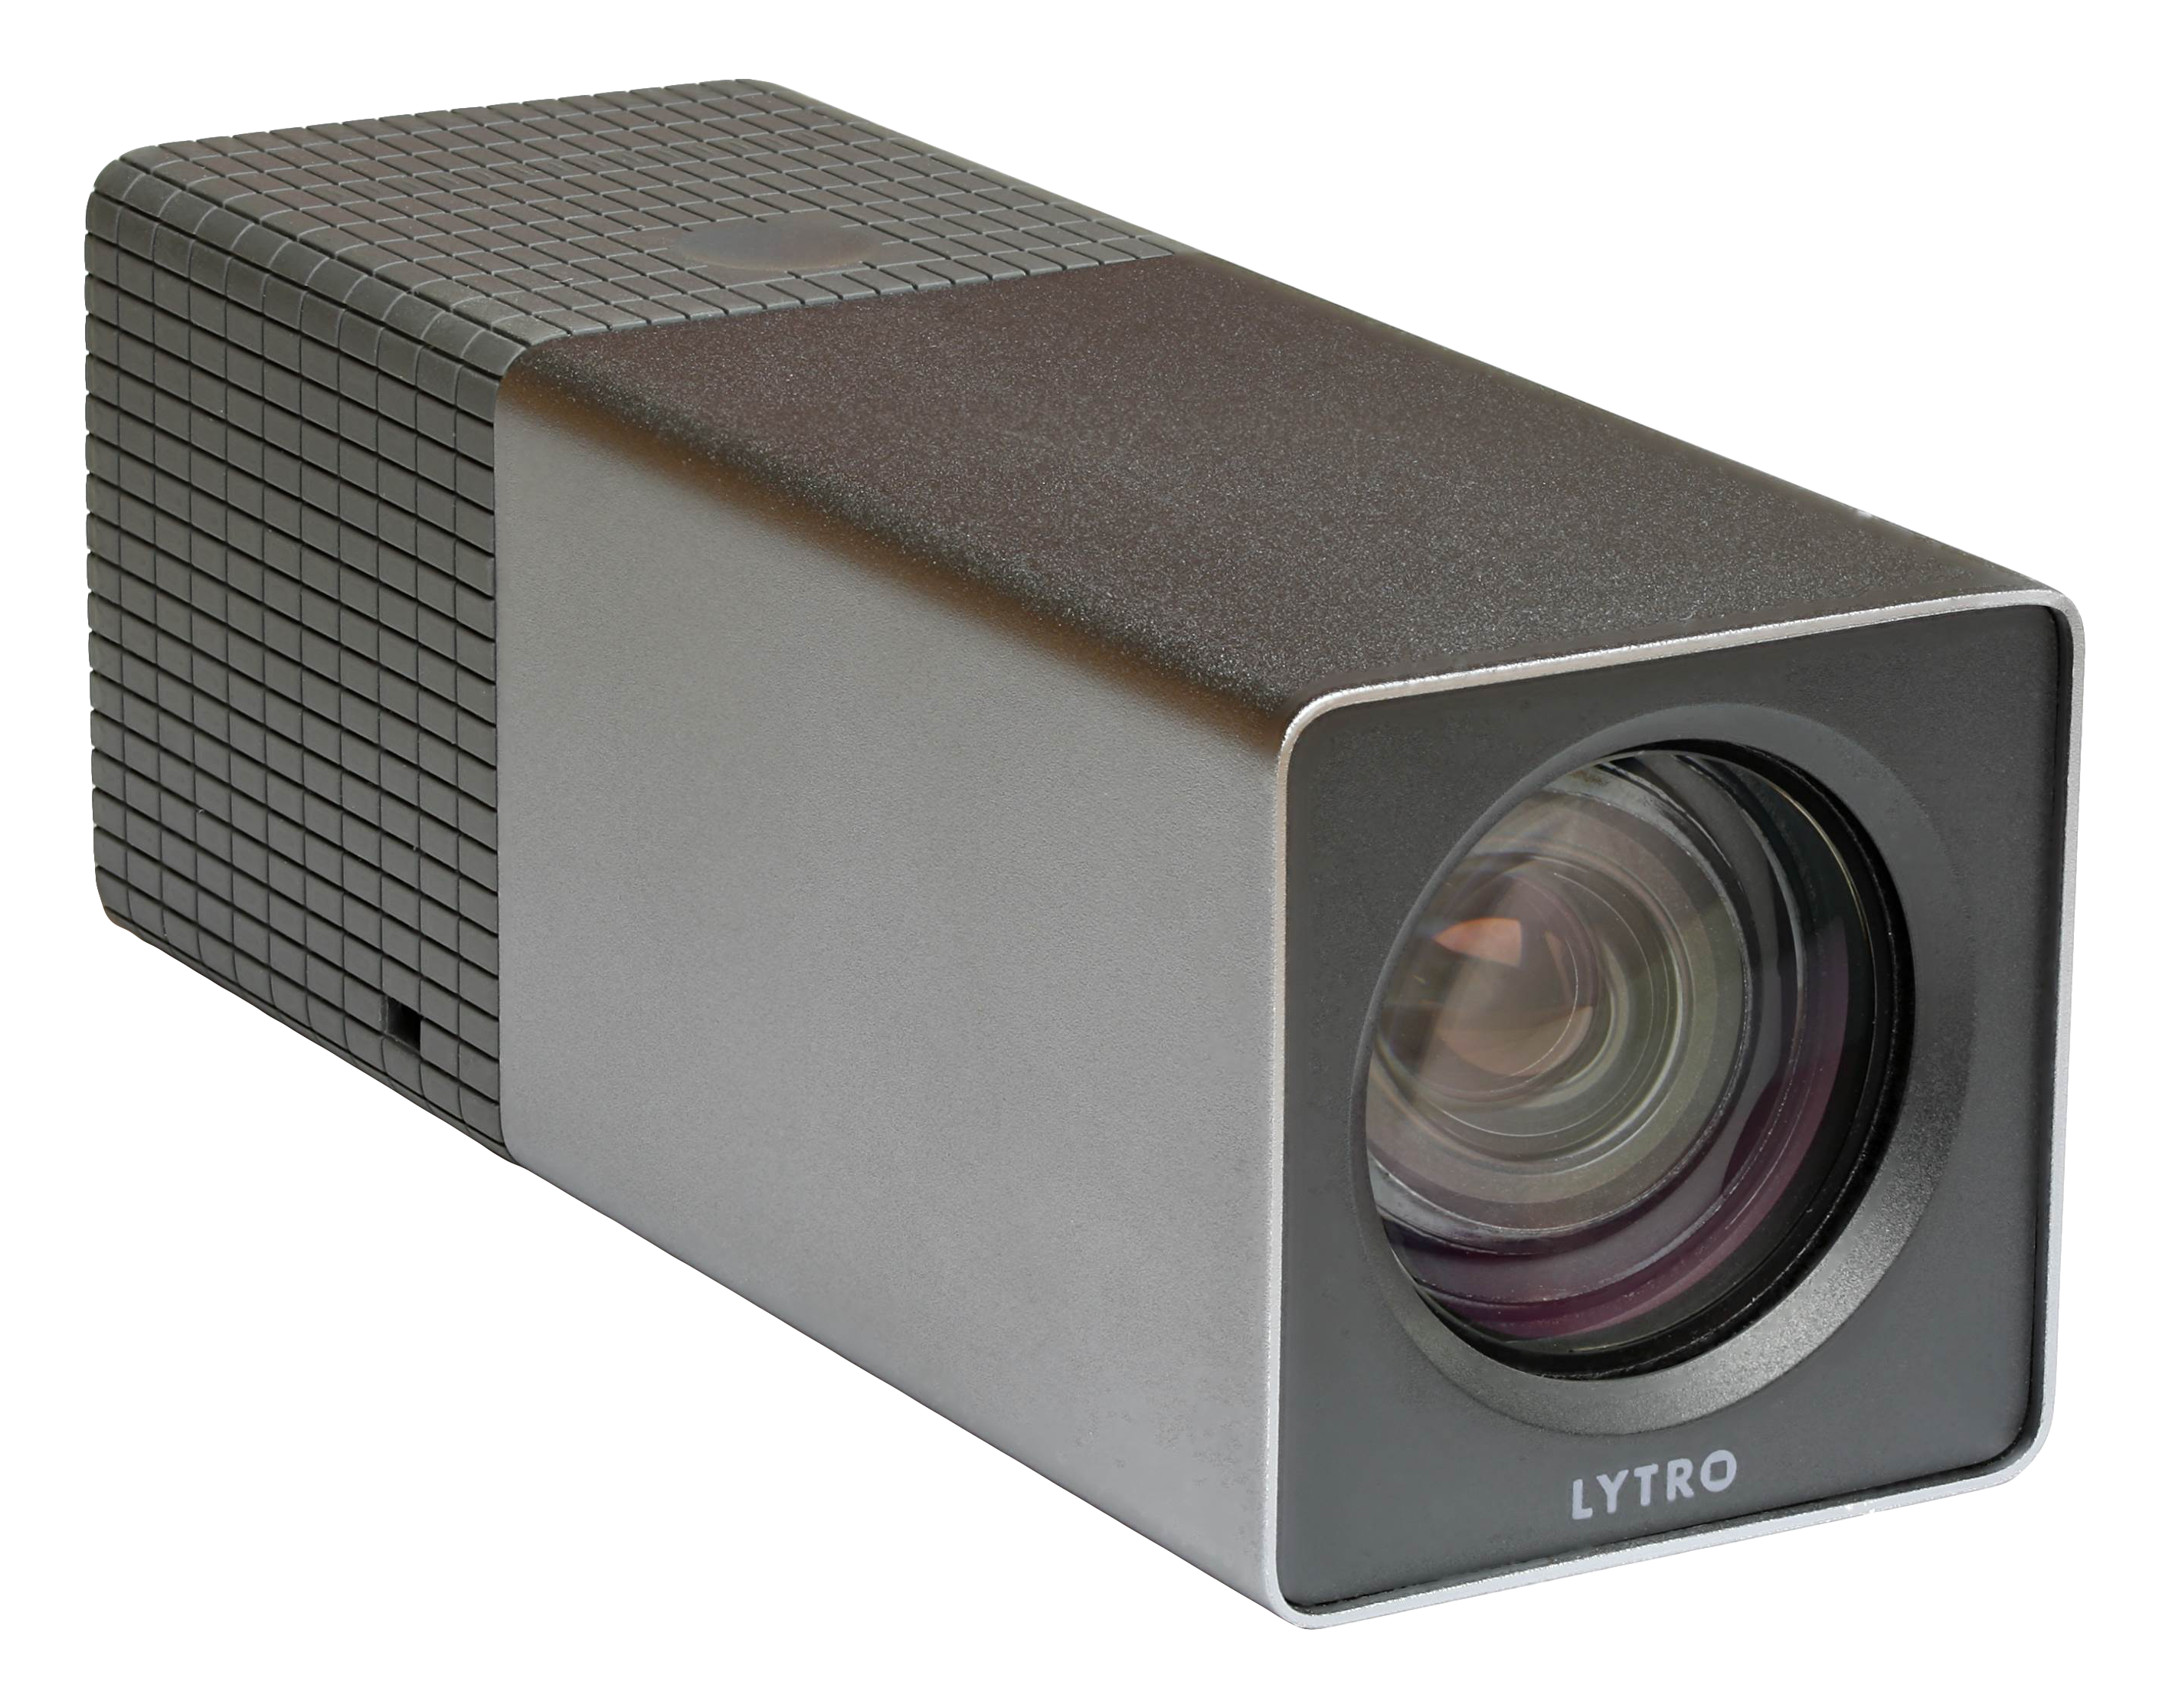
\includegraphics[height = 3.1cm]{images/Lytro_Light_Field_Camera-front_background_removed.png}}
	\end{center}
	
\end{frame}

\begin{frame}[fragile]
	\frametitle{Re-Parameterization to Global Coordinates}
	
	\begin{center}
		\visible<1,2>{\documentclass{standalone}
\usepackage{tikz}

\begin{document}
	
	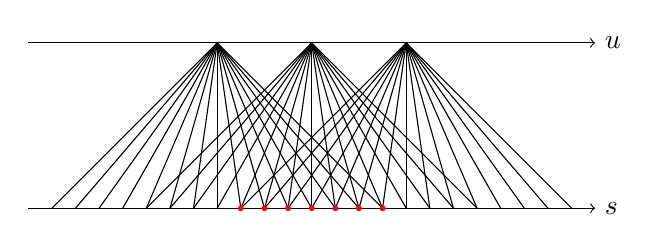
\begin{tikzpicture}[scale = 0.3]
		
		\draw[->] (-9, 0) -- (15, 0);
		\draw[->] (-9, 7) -- (15, 7);
		
		\node[right] at (15, 0) {$s$};
		\node[right] at (15, 7) {$u$};
		
		\draw (-1, 7) -- (-8, 0);
		\draw (-1, 7) -- (-7, 0);
		\draw (-1, 7) -- (-6, 0);
		\draw (-1, 7) -- (-5, 0);
		\draw (-1, 7) -- (-4, 0);
		\draw (-1, 7) -- (-3, 0);
		\draw (-1, 7) -- (-2, 0);
		\draw (-1, 7) -- (-1, 0);
		\draw (-1, 7) -- (0, 0);
		\draw (-1, 7) -- (1, 0);
		\draw (-1, 7) -- (2, 0);
		\draw (-1, 7) -- (3, 0);
		\draw (-1, 7) -- (4, 0);
		\draw (-1, 7) -- (5, 0);
		\draw (-1, 7) -- (6, 0);
		
		\draw (3, 7) -- (-4, 0);
		\draw (3, 7) -- (-3, 0);
		\draw (3, 7) -- (-2, 0);
		\draw (3, 7) -- (-1, 0);
		\draw (3, 7) -- (0, 0);
		\draw (3, 7) -- (1, 0);
		\draw (3, 7) -- (2, 0);
		\draw (3, 7) -- (3, 0);
		\draw (3, 7) -- (4, 0);
		\draw (3, 7) -- (5, 0);
		\draw (3, 7) -- (6, 0);
		\draw (3, 7) -- (7, 0);
		\draw (3, 7) -- (8, 0);
		\draw (3, 7) -- (9, 0);
		\draw (3, 7) -- (10, 0);
		
		\draw (7, 7) -- (0, 0);
		\draw (7, 7) -- (1, 0);
		\draw (7, 7) -- (2, 0);
		\draw (7, 7) -- (3, 0);
		\draw (7, 7) -- (4, 0);
		\draw (7, 7) -- (5, 0);
		\draw (7, 7) -- (6, 0);
		\draw (7, 7) -- (7, 0);
		\draw (7, 7) -- (8, 0);
		\draw (7, 7) -- (9, 0);
		\draw (7, 7) -- (10, 0);
		\draw (7, 7) -- (11, 0);
		\draw (7, 7) -- (12, 0);
		\draw (7, 7) -- (13, 0);
		\draw (7, 7) -- (14, 0);
		
		\draw[fill, red] (0, 0) circle [radius = 0.1];
		\draw[fill, red] (1, 0) circle [radius = 0.1];
		\draw[fill, red] (2, 0) circle [radius = 0.1];
		\draw[fill, red] (3, 0) circle [radius = 0.1];
		\draw[fill, red] (4, 0) circle [radius = 0.1];
		\draw[fill, red] (5, 0) circle [radius = 0.1];
		\draw[fill, red] (6, 0) circle [radius = 0.1];
	\end{tikzpicture}
	
\end{document}}
		\visible<2>{
			
\begin{tikzpicture}
				\draw[->, red, line width = 0.075cm] (0, 0) -- (0, -0.7);
			\end{tikzpicture}
		}	
		\visible<2>{\documentclass{standalone}
\usepackage{tikz}

\begin{document}
	
	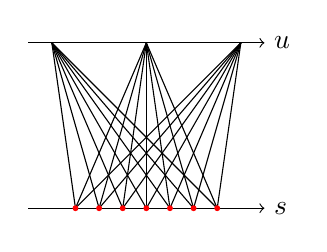
\begin{tikzpicture}[scale = 0.3]
		
		\draw[->] (-2, 0) -- (8, 0);
		\draw[->] (-2, 7) -- (8, 7);
		
		\node[right] at (8, 0) {$s$};
		\node[right] at (8, 7) {$u$};
		
		\draw (-1, 7) -- (0, 0);
		\draw (-1, 7) -- (1, 0);
		\draw (-1, 7) -- (2, 0);
		\draw (-1, 7) -- (3, 0);
		\draw (-1, 7) -- (4, 0);
		\draw (-1, 7) -- (5, 0);
		\draw (-1, 7) -- (6, 0);
		
		\draw (3, 7) -- (0, 0);
		\draw (3, 7) -- (1, 0);
		\draw (3, 7) -- (2, 0);
		\draw (3, 7) -- (3, 0);
		\draw (3, 7) -- (4, 0);
		\draw (3, 7) -- (5, 0);
		\draw (3, 7) -- (6, 0);
		
		\draw (7, 7) -- (0, 0);
		\draw (7, 7) -- (1, 0);
		\draw (7, 7) -- (2, 0);
		\draw (7, 7) -- (3, 0);
		\draw (7, 7) -- (4, 0);
		\draw (7, 7) -- (5, 0);
		\draw (7, 7) -- (6, 0);
		
		\draw[fill, red] (0, 0) circle [radius = 0.1];
		\draw[fill, red] (1, 0) circle [radius = 0.1];
		\draw[fill, red] (2, 0) circle [radius = 0.1];
		\draw[fill, red] (3, 0) circle [radius = 0.1];
		\draw[fill, red] (4, 0) circle [radius = 0.1];
		\draw[fill, red] (5, 0) circle [radius = 0.1];
		\draw[fill, red] (6, 0) circle [radius = 0.1];
		
	\end{tikzpicture}
	
\end{document}}
	\end{center}
\end{frame}

\begin{frame}[fragile]
	\frametitle{Re-Parameterization to Global Coordinates}
	
	\begin{center}
		\begin{tabular}{c p{0.5cm} c}
			Raw & & Rectified \\
			\fbox{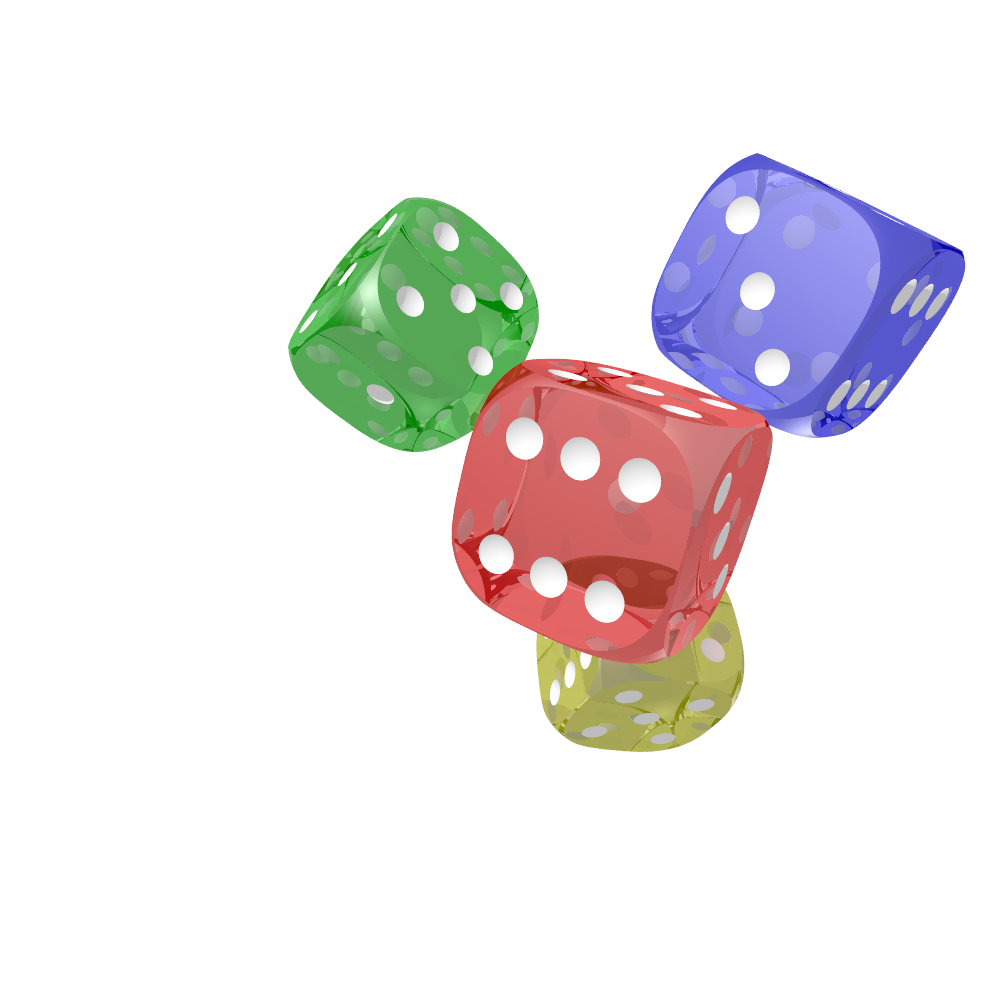
\includegraphics[height=5cm]{images/rectification/dice000_raw}}
			& &\fbox{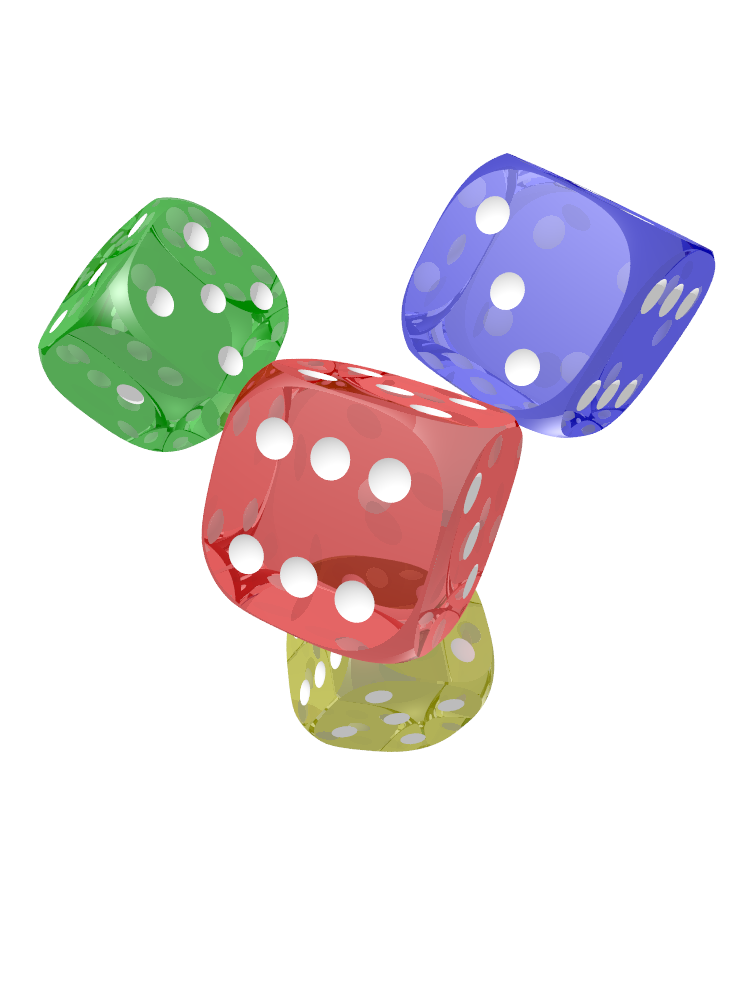
\includegraphics[height=5cm]{images/rectification/dice000_rectified}}
		\end{tabular}
	\end{center}
\end{frame}

\begin{frame}[fragile]
	\frametitle{Re-Parameterization to Global Coordinates}
	
	\begin{center}
		\begin{tabular}{c p{0.5cm} c}
			Raw & & Rectified \\
			\fbox{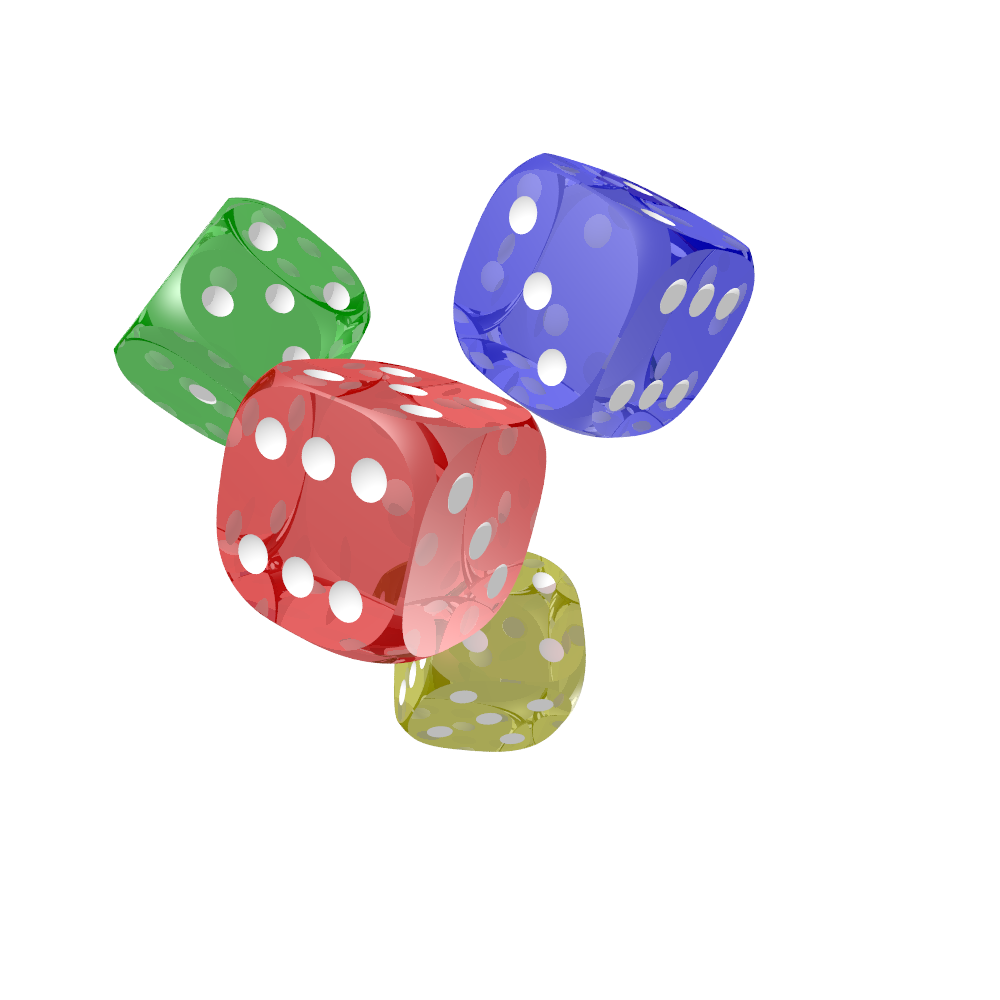
\includegraphics[height=5cm]{images/rectification/dice499_raw}}
			& &\fbox{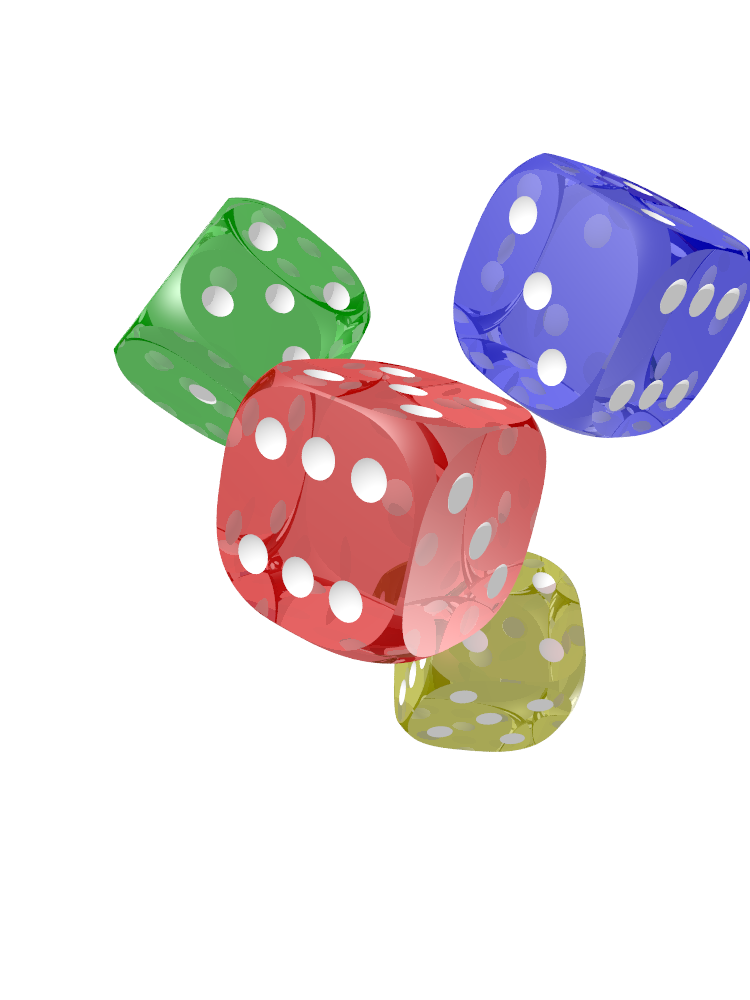
\includegraphics[height=5cm]{images/rectification/dice499_rectified}}
		\end{tabular}
	\end{center}
\end{frame}

\section{Attenuation Display}

\begin{frame}[fragile]
	\frametitle{The Beer-Lambert Law}
	\begin{center}
		\includegraphics<1>[height = 7cm]{figures/beer-lambert/lambert-beer-law_illustration.pdf}
		\includegraphics<2>[height = 7cm]{figures/beer-lambert/lambert-beer-law_layers1.pdf}
		\includegraphics<3>[height = 7cm]{figures/beer-lambert/lambert-beer-law_layers2.pdf}
		\includegraphics<4>[height = 7cm]{figures/beer-lambert/lambert-beer-law_layers3.pdf}
	\end{center}
\end{frame}

\begin{frame}[fragile]
	\frametitle{Display Architecture}
	\begin{center}
		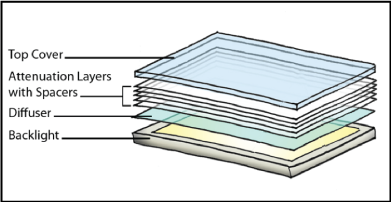
\includegraphics[width=10cm]{images/display_architecture.png}
	\end{center}
\end{frame}

\begin{frame}[fragile]
	\frametitle{Light Transmission}
	\vspace{1cm}
	\begin{columns}[onlytextwidth]
		\column{0.45\textwidth} 
			\documentclass{standalone}
\usepackage{tikz}
\usepackage{xcolor}
\usetikzlibrary{intersections}

\begin{document}
	
	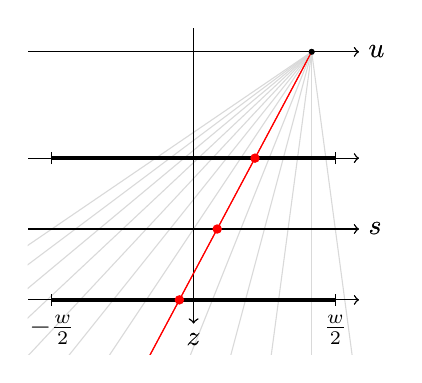
\begin{tikzpicture}[scale = 0.15,
						one end extended/.style = {shorten <= -#1},
	 					one end extended/.default = 1cm,
	 					]
	
		\colorlet{lightgray}{gray!30}
		
		% Top and bottom layer planes
		\draw[->, name path = bottomLayer] (-14, -6) -- (14, -6);
		\draw[->, name path = topLayer] (-14, 6) -- (14, 6);
					
		% Camera plane
		\draw[->] (-14, 15) -- (14, 15);
		\node[right] at (14, 15) {$u$};
		
		% Sensor plane
		\draw[<-, name path = sensor] (14, 0) -- (-14, 0);
		\node[right] at (14, 0) {$s$};
			
		% Camera position marker
		\coordinate (cameraCenter) at (10, 15);
		\fill[black] (cameraCenter) circle[radius = 0.25];
				
		\draw[ultra thick] (-12, -6) -- (12, -6);
		\draw[ultra thick] (-12, 6) -- (12, 6);
				
		% z-axis
		\draw[->] (0, 15 + 2) -- (0, -8);
		\node[below] at (0, -8) {$z$};
		
		% Save current bounding box to clip light rays
		\coordinate (NE) at (current bounding box.north east);
		\coordinate (SW) at (current bounding box.south west);
		\clip (SW) rectangle (NE);
		
		% Rays and intersections
		\coordinate (s0) at (-12, 0);
		\coordinate (s1) at (-10, 0);
		\coordinate (s2) at (-8, 0);
		\coordinate (s3) at (-6, 0);
		\coordinate (s4) at (-4, 0);
		\coordinate (s5) at (-2, 0);
		\coordinate (s6) at (0, 0);
		\coordinate (s7) at (2, 0);
		\coordinate (s8) at (4, 0);
		\coordinate (s9) at (6, 0);
		\coordinate (s10) at (8, 0);
		\coordinate (s11) at (10, 0);
		\coordinate (s12) at (12, 0);
		
		\draw[one end extended = 10cm, lightgray] (s0) -- (cameraCenter);
		\draw[one end extended = 10cm, lightgray] (s1) -- (cameraCenter);
		\draw[one end extended = 10cm, lightgray] (s2) -- (cameraCenter);
		\draw[one end extended = 10cm, lightgray] (s3) -- (cameraCenter);
		\draw[one end extended = 10cm, lightgray] (s4) -- (cameraCenter);
		\draw[one end extended = 10cm, lightgray] (s5) -- (cameraCenter);
		\draw[one end extended = 10cm, lightgray] (s6) -- (cameraCenter);
		\draw[one end extended = 10cm, red, name path = ray] (s7) -- (cameraCenter);
		\draw[one end extended = 10cm, lightgray] (s8) -- (cameraCenter);
		\draw[one end extended = 10cm, lightgray] (s9) -- (cameraCenter);
		\draw[one end extended = 10cm, lightgray] (s10) -- (cameraCenter);
		\draw[one end extended = 10cm, lightgray] (s11) -- (cameraCenter);
		\draw[one end extended = 10cm, lightgray] (s12) -- (cameraCenter);
		
		% Draw lines of coordinate system again on top of rays
		\draw[->] (-14, -6) -- (14, -6);
		\draw[->] (-14, 6) -- (14, 6);
		\draw[->] (-14, 15) -- (14, 15);
		\node[right] at (14, 15) {$u$};
		\draw[<-] (14, 0) -- (-14, 0);
		\node[right] at (14, 0) {$s$};
		\draw[ultra thick] (-12, -6) -- (12, -6);
		\draw[ultra thick] (-12, 6) -- (12, 6);
		\draw[->] (0, 15 + 2) -- (0, -8);
		\node[below] at (0, -8) {$z$};
		
		\draw[one end extended = 10cm, red, name path = ray] (s7) -- (cameraCenter);
		\fill[black] (cameraCenter) circle[radius = 0.25];
		
		% Intersection markers
		\fill[red] (-1.2, -6) circle[radius = 0.4];
		\fill[red] (2, 0) circle[radius = 0.4];
		\fill[red] (5.2, 6) circle[radius = 0.4];
							
		% Width markers
		\draw (-12, -0.5 + 6) -- (-12, 0.5 + 6);
		\draw (12, -0.5 + 6) -- (12, 0.5 + 6);
		\draw (-12, -0.5 - 6) -- (-12, 0.5 - 6);
		\draw (12, -0.5 - 6) -- (12, 0.5 - 6);
		\node[below] at (-12, -0.5 - 6) {$-\frac{w}{2}$};
		\node[below] at (12, -0.5 - 6) {$\frac{w}{2}$};
		
	\end{tikzpicture}
	
\end{document}
		\column{0.4\textwidth}
			\begin{equation*}
				L_m = L_0 \prod_{n=1}^{N} t^{(n)} (h(m, n)) 
			\end{equation*}
			\begin{itemize}[<alert@+>]
			    \item[$L_m$] Color of ray $m$
			    \item[$t$] Transmission
			    \item[$h$] Intersection 
			\end{itemize}
	\end{columns}
	\vspace{1cm}
	\begin{center}
		\visible<4>{\alert{From now on: $L_0 = 1$}}
	\end{center}
\end{frame}

\begin{frame}[fragile]
	\frametitle{From Transmission to Absorbance}
	
	\begin{itemize}[<+- | alert@+>]
		\item Transmission values unknown
		\item Solve equations simultaneously for all rays
		\item This is hard
		\item Transform to log-domain
		\item Solve for absorbance
	\end{itemize}
	\visible<1,2,3,4,5>{
	\begin{equation*}
		L_m = \prod_{n=1}^{N} t^{(n)} (h(m, n)) 
	\end{equation*}}
	\visible<4,5>{
	\begin{center}
		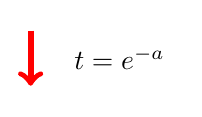
\begin{tikzpicture}
			\draw[->, red, line width = 0.075cm] (0, 0) -- (0, -0.7) node[midway, right, xshift=0.4cm, black] {$t = e^{-a}$};
		\end{tikzpicture}
	\end{center}
	\begin{equation*}
		\text{log}(L_m) = - \sum_{n=1}^{N} a^{(n)} (h(m, n)) 
	\end{equation*}}
	
\end{frame}

\begin{frame}[fragile]
	\frametitle{Ray Casting}
	
	\begin{itemize}[<alert@+>]
		\item One linear constraint per ray
		\item Create a big matrix $P$
		\item Matrix encodes intersections
	\end{itemize}
	\vspace{2cm}
	\begin{equation*}
			\text{log}(L_m) = -\sum_{n=1}^{N} a^{(n)} (h(m, n)) 
	\end{equation*}
	
\end{frame}

\begin{frame}[fragile]
	\frametitle{Ray Casting}
	$
		P = 
		\begin{blockarray}{lcccccccccc}
		    				& \alpha_1 	& \alpha_2 	& \alpha_3 	& \alpha_4 	& \alpha_5 	& \alpha_6 	& \alpha_7 	& \alpha_8 	& \alpha_9 	& \alpha_{10}	\\
		    \begin{block}{l(ccccc|ccccc@{\hspace*{5pt}})}
			  \bar{L}_1 	& 	 		& 			& 	1		& 			& 			& 	1		&			&			&			&				\\
			  \bar{L}_2 	& 			& 			& 			& 	1		& 			& 	1		&			&			&			&				\\
			  \bar{L}_3 	& 	1		& 			& 			& 			& 			& 			&	1		&			&			&				\\
			  \bar{L}_4 	& 			& 	1		& 			& 			& 			& 			&			&			&	1		&				\\
			  \cline{2-11}
			  \bar{L}_5 	& 			& 			& 			& 			& 	1		& 			&			&			&	1		&				\\
			  \bar{L}_6 	& 			& 			& 	1		& 			& 			& 1			&			&			&			&				\\
			  \bar{L}_7 	& 		1	& 			& 			& 			& 			& 			&			&			&	1		&				\\
			  \bar{L}_8 	& 			& 			& 			& 	 		& 	1		& 			&	1		&			&			&				\\
			  \cline{2-11}
			  \bar{L}_9 	& 			& 	1		& 			& 			& 			& 			&	1		&			& 			&				\\
			  \bar{L}_{10} 	& 			& 			& 			& 		1	& 			& 			&			&	1		&			&				\\
			  \bar{L}_{11} 	& 			& 			& 	1		& 			& 			& 			&			&			&	1		&				\\
			  \bar{L}_{12} 	& 			& 	1		& 			& 	 		& 			& 			&			&			&	1		&				\\			  
		    \end{block}
		\end{blockarray}
	$
\end{frame}

\begin{frame}[fragile]
	\frametitle{The Equation}
	
	\begin{equation*}
		\text{log}(L) = - P \alpha
	\end{equation*}
	
	\begin{itemize}[<alert@+>]
		\item $\text{log}(L)$ Vectorized log light field
		\item $\alpha$ Vector holding unkowns
	\end{itemize}
\end{frame}

\begin{frame}[fragile]
	\frametitle{Optimization Problem}
	
	\begin{equation*}
		\begin{aligned}
			& \underset{\alpha}{\text{argmin}} 	& & \left\lVert P \alpha + \log(L) \right\rVert ^2 \\
			& \text{subject to} 				& & \alpha \geq 0.
		\end{aligned}
	\end{equation*}
	
	\begin{itemize}
		\item Proposed by \cite{WetzsteinTomo}
		\item System is overdetermined
		\item Need iterative solver
	\end{itemize}
\end{frame}

\begin{frame}[fragile]
	\frametitle{The Constraint $\alpha \geq 0$}
	
	\begin{itemize}
		\item Negative absorption ($\alpha < 0$) is physically not possible
		\item The theoretical model supports negative absorption
		\item Constraint reduces the space of possible solutions
	\end{itemize}
\end{frame}

\begin{frame}[fragile]
	\frametitle{Examples}
	
	\begin{center}
		\begin{tabular}{cc}
			\raisebox{-.5\height}{
				\begin{overpic}[width=5cm,tics=10]{images/layers_and_projections/legotruck/1}
					\put (63, 60) {bottom}
				\end{overpic}
			} & 
			\raisebox{-.5\height}{
				\begin{overpic}[width=5cm,tics=10]{images/layers_and_projections/legotruck/2}
					\put (65, 60) {middle}
				\end{overpic}
			} 
			\\
			\raisebox{-.5\height}{
				\begin{overpic}[width=5cm,tics=10]{images/layers_and_projections/legotruck/3}
					\put (78, 60) {top}
				\end{overpic}
			} & 
			\begin{tabular}{@{}c@{}}
				$6 \times 6 \times 480 \times 640$ \\
				$\sim$ 10 minutes
			\end{tabular} 
			\\
		\end{tabular}
	\end{center}
	
	% Lego truck layers
	% No tiling
	
\end{frame}

\begin{frame}[fragile]
	\frametitle{Examples}
	
	% Tarot cards
	% No tiling
	
\end{frame}

\begin{frame}[fragile]
	\frametitle{Examples}
	
	% Lytro rubik's cube
	% No tiling
	
	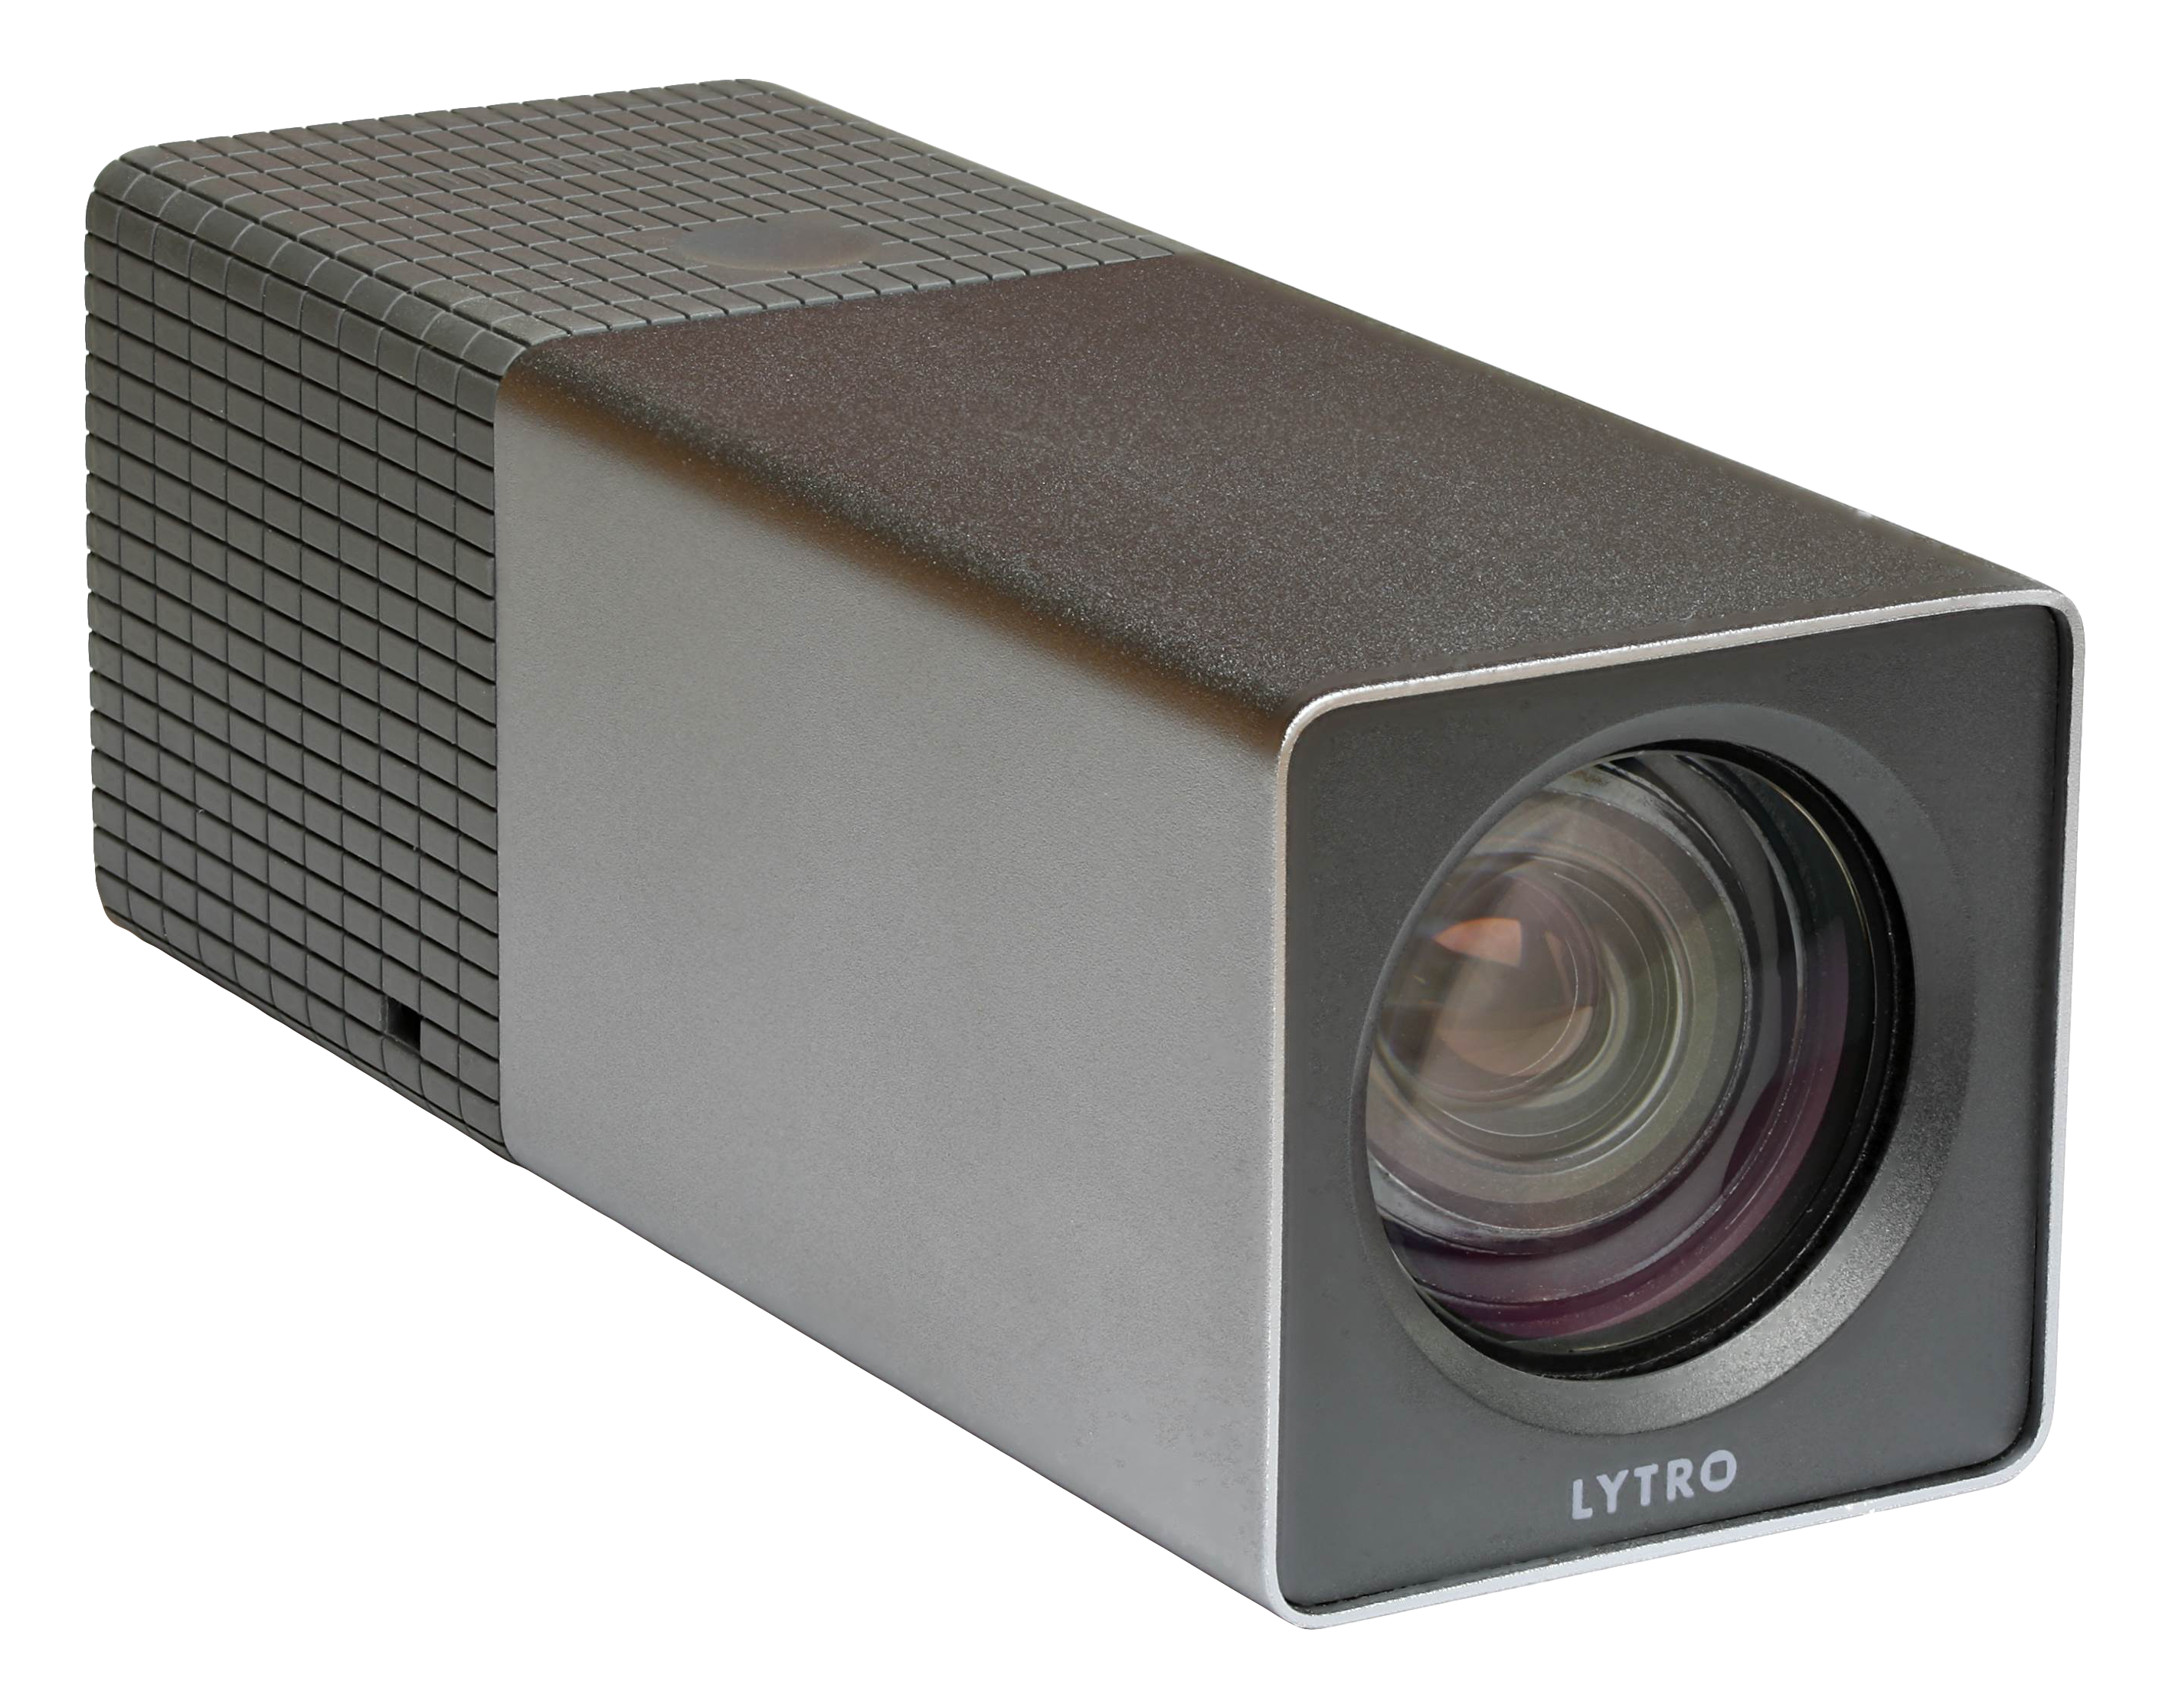
\includegraphics[height = 2cm]{images/Lytro_Light_Field_Camera-front_background_removed}
\end{frame}

\begin{frame}[fragile]
	\frametitle{Attenuator Tiling}
	
	\begin{enumerate}
		\item Slice attenuator into smaller pieces
		\item Solve optimization problem for every slice
		\item Reconnect the slices
	\end{enumerate}
	
	\vspace{1cm}
	
	\begin{center}
		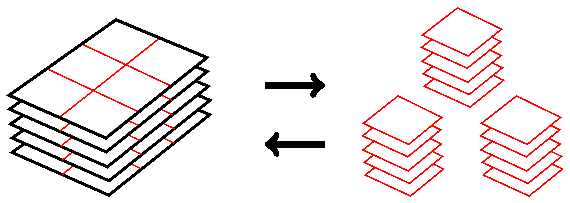
\includegraphics[height = 3cm]{figures/slicing_attenuator/tiling_overview.pdf}
	\end{center}
\end{frame}

\begin{frame}[fragile]
	\frametitle{Attenuator Tiling}

	\begin{itemize}
		\item Problem: Rays can overlap with multiple slices at borders
		\item Slices need to overlap
		\item Blend slices with mask
	\end{itemize}
\end{frame}

\begin{frame}[fragile]
	\frametitle{The Finished Product}
	\begin{center}
		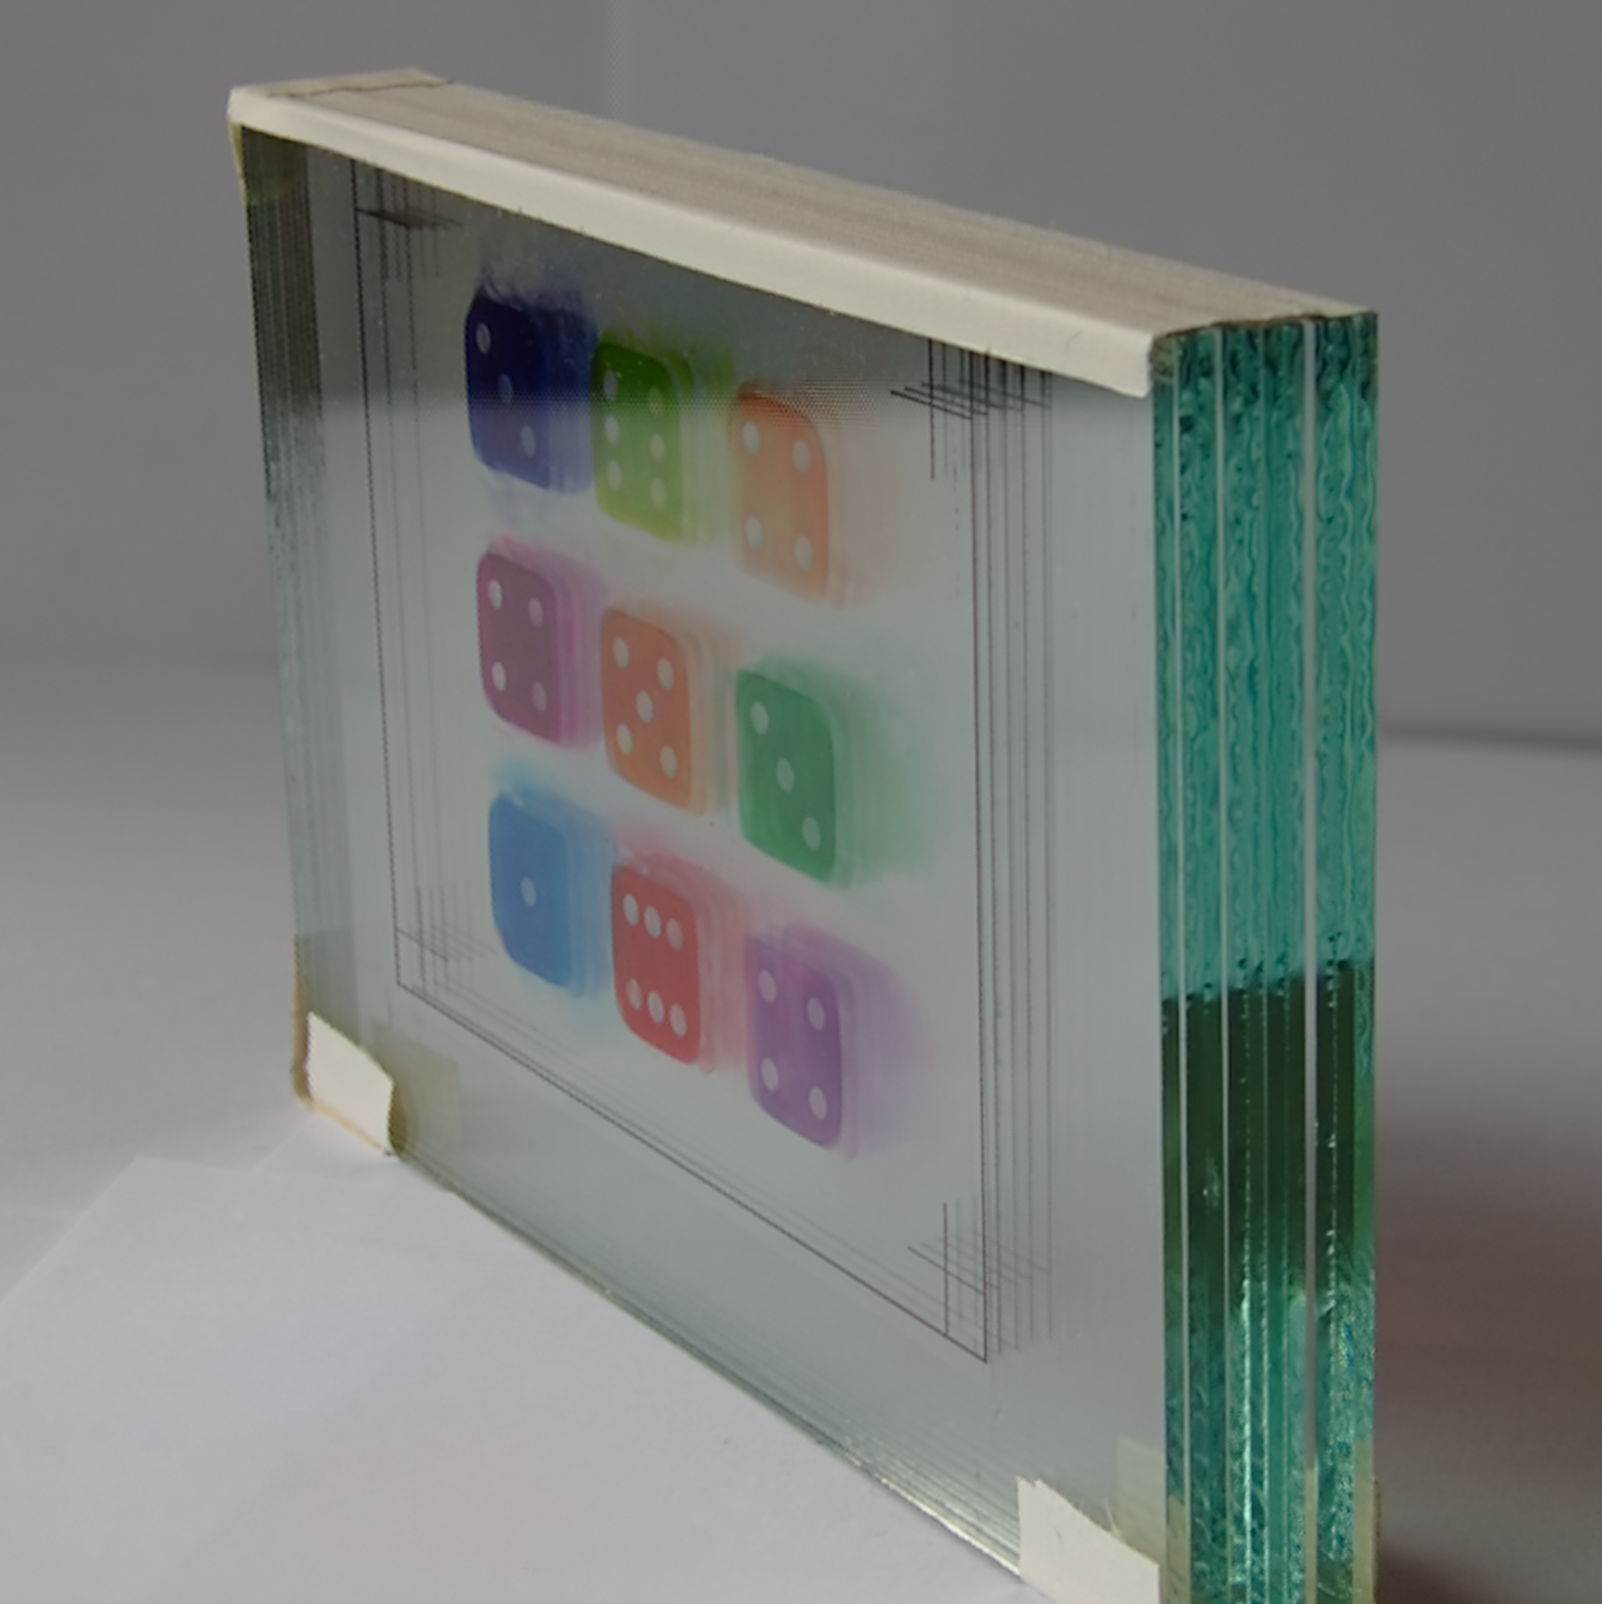
\includegraphics[height=4cm]{images/glass_plates_front_view_cropped}
		\hspace{1cm}
		\includegraphics[height=4cm]{images/raw_backlight_from_top}
	\end{center}
\end{frame}

\begin{frame}[fragile]
	\frametitle{The Finished Product}
	\begin{center}
		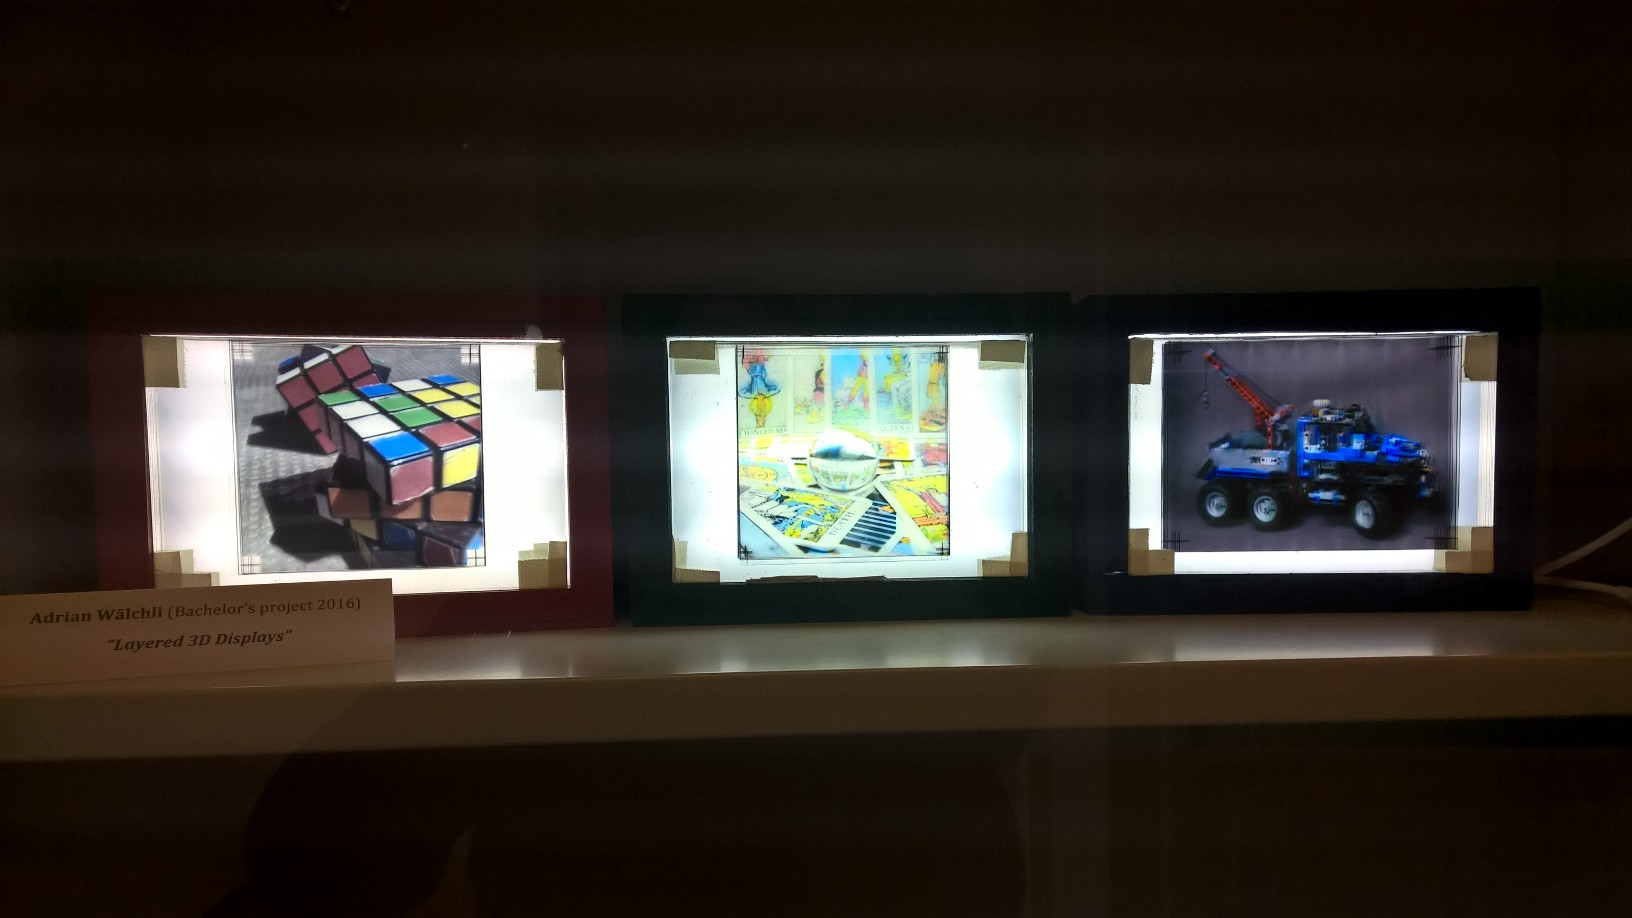
\includegraphics[width=9cm]{images/all_displays_on}
	\end{center}
\end{frame}

\begin{frame}[fragile]
	\frametitle{Questions}
	
	\begin{itemize}
		\item Impact of more layers?
		\item Does thickness of display matter?
		\item What are the limitations?
	\end{itemize}
\end{frame}

\section{Assessment}

\begin{frame}[fragile]
	\frametitle{Epipolar Plane Geometry}
	\begin{center}
		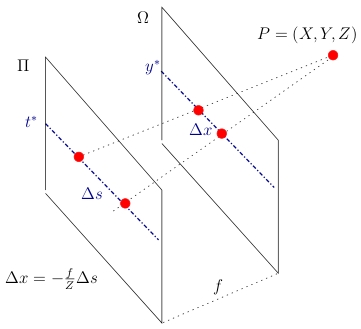
\includegraphics[height = 6cm]{images/lf_geometry.jpg}
	\end{center}
\end{frame}

\begin{frame}[fragile]
	\frametitle{Epipolar Plane Image}
	\begin{center}
		\begin{tikzpicture}
			\draw[->] (0, 0) -- (3, 0) node[midway, above] {$u$};
		\end{tikzpicture}
		
		\vspace{0.1cm}
		
		\frame{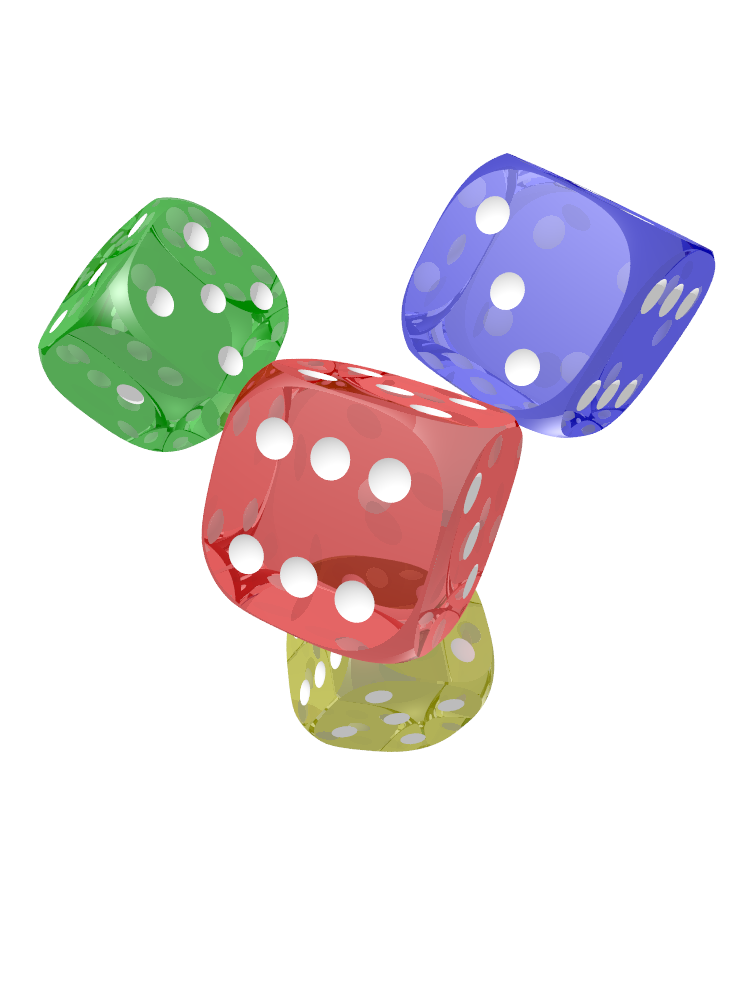
\includegraphics[width = 1cm]{images/epi_dice/dice000.png}}
		\hspace{0.1cm}
		\frame{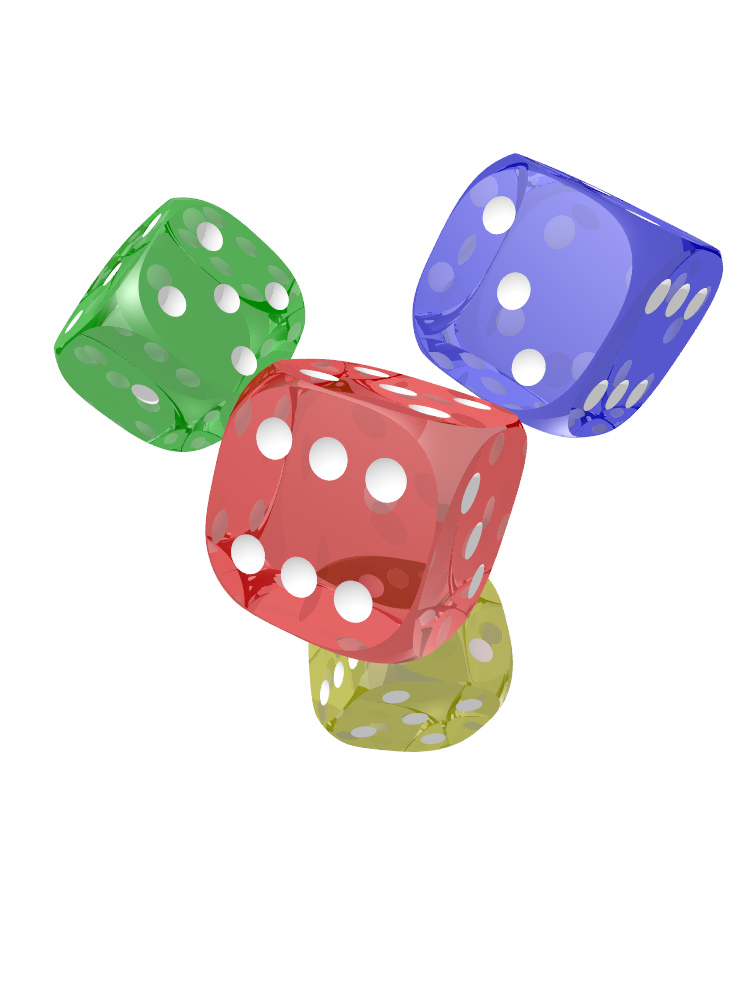
\includegraphics[width = 1cm]{images/epi_dice/dice099.png}}
		\hspace{0.1cm}
		\frame{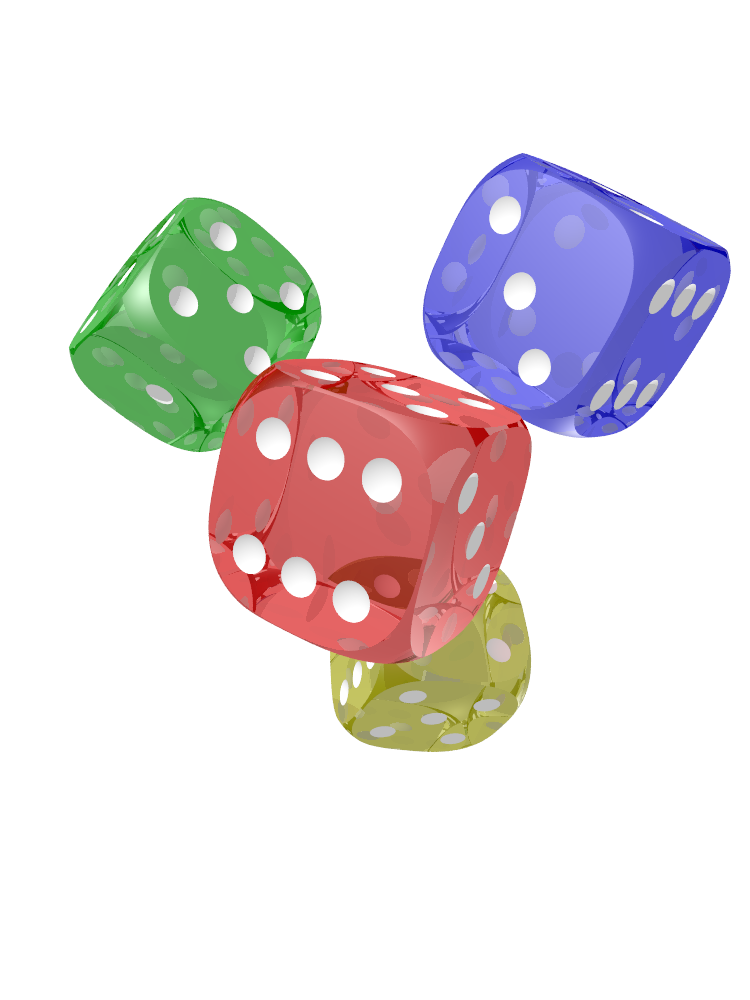
\includegraphics[width = 1cm]{images/epi_dice/dice199.png}}
		\hspace{0.1cm}
		\frame{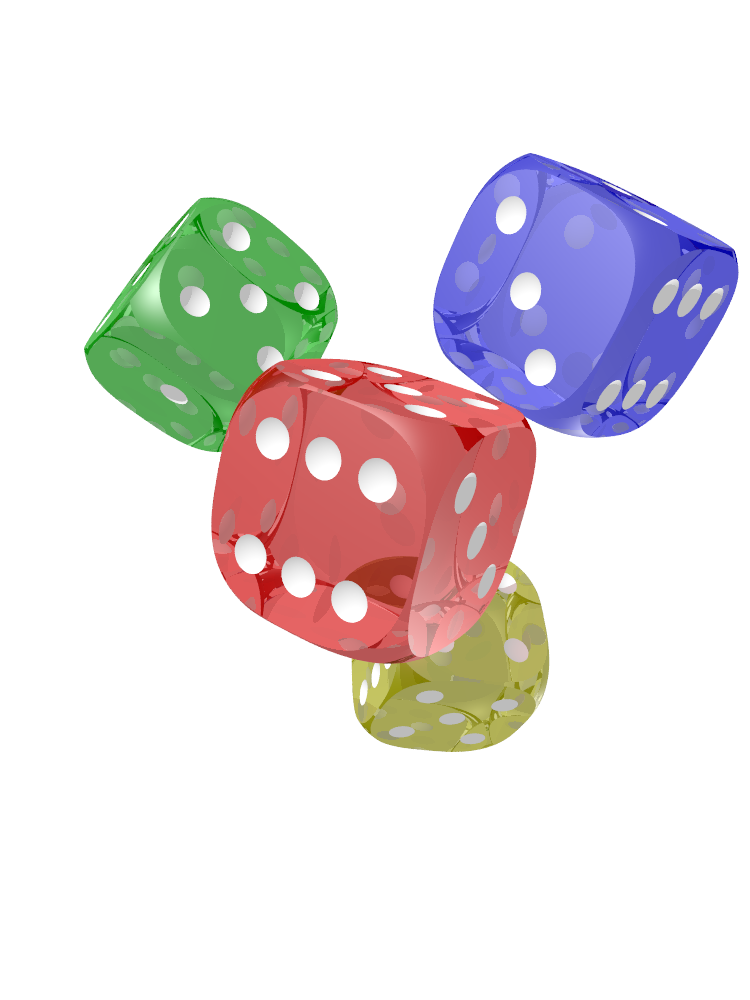
\includegraphics[width = 1cm]{images/epi_dice/dice299.png}}
		\hspace{0.1cm}
		\frame{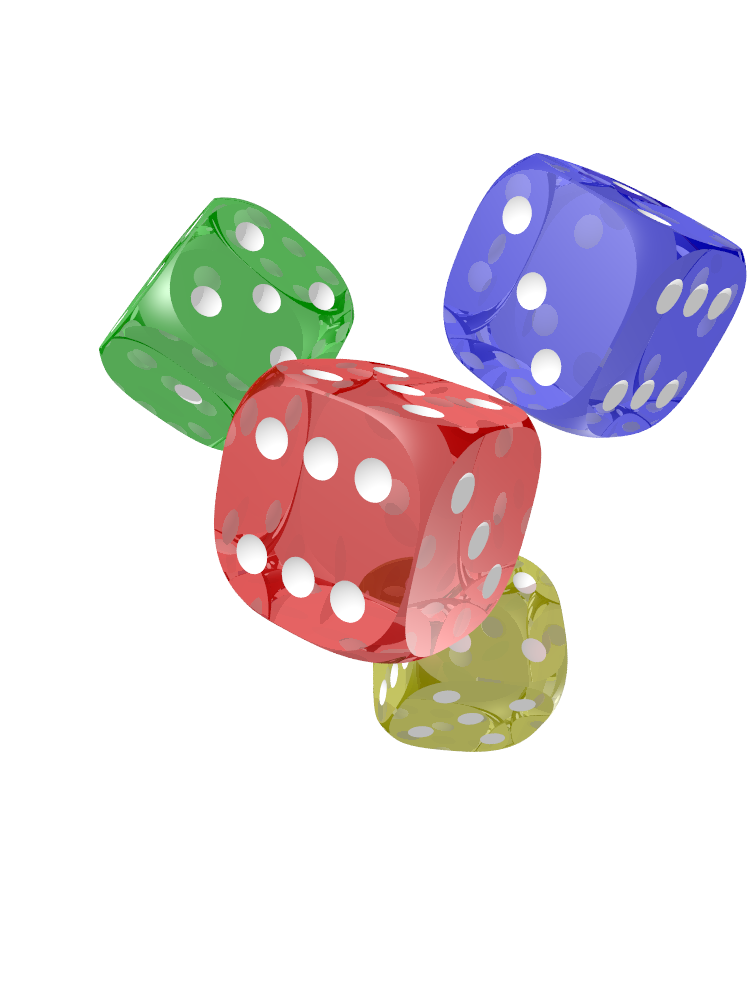
\includegraphics[width = 1cm]{images/epi_dice/dice399.png}}
		\hspace{0.1cm}
		\frame{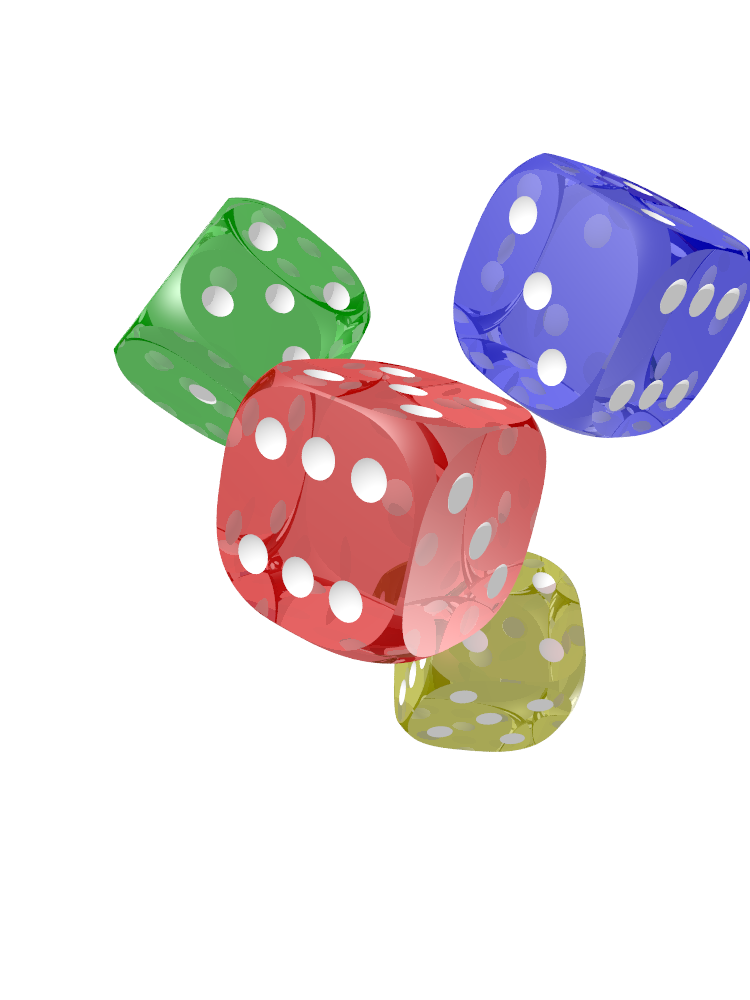
\includegraphics[width = 1cm]{images/epi_dice/dice499.png}}
	\end{center}
	
	\vspace{0.5cm}
	
	\begin{columns}[onlytextwidth]
		\column{0.5\textwidth}
			\documentclass{standalone}
\usepackage{tikz}
\usepackage{pgfplots}

\begin{document}
	\begin{tikzpicture}[baseline]
		\begin{axis}[	scale only axis,
						height = 3.2cm,
						ylabel near ticks,
						xlabel near ticks, 
						ticks = none, 
						enlargelimits = true, 
						axis on top, 
						axis equal image,
						axis lines = left,
						xlabel = {$x$},
						ylabel = {$y$} 
					]
	
			\addplot graphics [xmin = 125, xmax = 875, ymin = 0, ymax = 615] {figures/epi_1x500x1000x1000/rectified/overview};
		
			\addplot[mark = none, black] coordinates {(0, 615 - 497) (1000, 615 - 497)};
			\addplot[mark = none, black] coordinates {(0, 615 - 236) (1000, 615 - 236)};
			
			\only<2>{\addplot[mark = none, red] coordinates {(0, 615 - 497) (1000, 615 - 497)};}
			\only<1>{\addplot[mark = none, red] coordinates {(0, 615 - 236) (1000, 615 - 236)};}
			
		\end{axis}
	\end{tikzpicture}	
\end{document}
		\column{0.5\textwidth}
			\only<1>{\documentclass{standalone}
\usepackage{tikz}
\usepackage{pgfplots}

\begin{document}
	\begin{tikzpicture}[baseline]
		\begin{axis}[	scale only axis,
						height = 2.8cm,
						xtick = {0, 1000}, 
						ytick = {0, 500},
						ylabel near ticks,
						xlabel near ticks, 
						ticks = none, 
						enlargelimits = true, 
						axis on top, 
						axis equal image,
						axis lines = left, 
						xlabel = {$x$}, 
						ylabel = {$u$}
					]
	
			% Add dummy line to set the size of the coordinate system
			\addplot[mark = none, white] coordinates {(0, 0) (1000, 0)};
	
			\addplot[plot graphics/node/.append style={yscale=-1,anchor=north west}] % Flip EPI vertically (MATLAB matrix)
					graphics [xmin = 125, xmax = 875, ymin = 0, ymax = 500] {epi_1x500x1000x1000/rectified/scanY=379};
		
		\end{axis}
	\end{tikzpicture}	
\end{document}}
			\only<2>{\documentclass{standalone}
\usepackage{tikz}
\usepackage{pgfplots}

\begin{document}
	\begin{tikzpicture}[baseline]
		\begin{axis}[	scale only axis,
						height = 3.2cm,
						xtick = {0, 1000}, 
						ytick = {0, 500},
						ylabel near ticks,
						xlabel near ticks, 
						ticks = none, 
						enlargelimits = true, 
						axis on top, 
						axis equal image,
						axis lines = left, 
						xlabel = {$x$}, 
						ylabel = {$u$}
					]
	
			% Add dummy line to set the size of the coordinate system
			\addplot[mark = none, white] coordinates {(0, 0) (1000, 0)};
	
			\addplot[plot graphics/node/.append style={yscale=-1,anchor=north west}] % Flip EPI vertically (MATLAB matrix)
					graphics [xmin = 125, xmax = 875, ymin = 0, ymax = 500] {figures/epi_1x500x1000x1000/rectified/scanY=641};
			
		\end{axis}
	\end{tikzpicture}	
\end{document}}
	\end{columns}
\end{frame}

\begin{frame}[fragile]
	\frametitle{Spectral Analysis}
	
	\begin{center}
		\documentclass{standalone}
\usepackage{tikz}
\usepackage{pgfplots}

\tikzset{align at bottom/.style={baseline=(current bounding box.south)}}

\begin{document} 
	\begin{tikzpicture}[scale = 0.27]
	
		\draw[->] (-5, 0) -- (5, 0) node[right] {$s$};
		\draw[<-] (-5, -5) -- (-5, 5) node[above] {$z$};
	
		\begin{scope}
			\clip (-5, -5) rectangle (5, 5);
			\draw[scale = 1, smooth, domain = -10 : 10, variable = \x, black, dashed] plot ({\x}, {3});
			\draw[scale = 1, smooth, domain = -10 : 10, variable = \x, black, dashed] plot ({\x}, {-2});
		\end{scope}
		
		\node[left] at (-5, 3) {$Z_\textrm{min}$};
		\node[left] at (-5, -2) {$Z_\textrm{max}$};
		
		\draw[ultra thick, blue] (0, 3) -- (2, 3);
		\draw[ultra thick, red] (-3, -2) -- (0, -2);
		
		% Phantom node for alignment
		\node[right, opacity = 0] at (-5, -5) {$s$};
		
	\end{tikzpicture}
\end{document}
		\hspace{1cm}
		\documentclass{standalone}
\usepackage{tikz}
\usepackage{pgfplots}

\tikzset{align at bottom/.style={baseline=(current bounding box.south)}}

\begin{document} 
	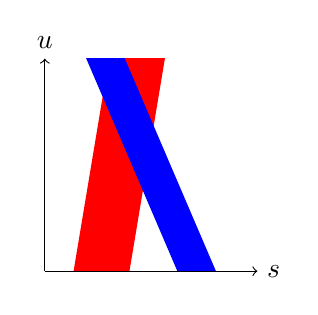
\begin{tikzpicture}[scale = 0.27]
	
		\begin{scope}
			\clip (-5, -5) rectangle (5, 5);
			\draw[scale = 1, smooth, variable = \x, red, line width = 0.7cm] plot ({\x}, { 12 / 2 * (\x + 1.5)});
			\draw[scale = 1, smooth, variable = \x, blue, line width = 0.45cm] plot ({\x}, { -7 / 3 * \x});
		\end{scope}
		
		\draw[->] (-5, -5) -- (5, -5) node[right] {$s$};
		\draw[->] (-5, -5) -- (-5, 5) node[above] {$u$};
		
	\end{tikzpicture}
\end{document}
	\end{center}
	
	\begin{equation*}
		\frac{\text{d}u}{\text{d}s} = \frac{z - Z_u}{z - Z_s}
	\end{equation*}
	
\end{frame}

\begin{frame}[fragile]
	\frametitle{Spectral Analysis}
	
	\begin{center}
		\documentclass{standalone}
\usepackage{tikz}
\usepackage{pgfplots}

\tikzset{align at bottom/.style={baseline=(current bounding box.south)}}

\begin{document}
	\begin{tikzpicture}[scale = 0.35]
	
		\begin{scope}
			\clip (-5, -5) rectangle (5, 5);
			%\node[anchor = center, inner sep = 0, opacity = 0.4] at (0, 0) {\includegraphics[width = 5cm]{../Figures/spectral_support/fft_red_and_blue.png}};
		\end{scope}
		
		\draw[->] (-5, 0) -- (5, 0) node[right] {$\xi_s$};
		\draw[->] (0, -5) -- (0, 5) node[above] {$\xi_u$};
		
		% Invisible dummy node for symmetric alignment with caption
		\node[left, opacity = 0] at (-5, 0) {$\xi_s$};
		
		\begin{scope}
			\clip (-5, -5) rectangle (5, 5);
			\draw[scale=1, smooth, domain = -10 : 10, variable = \x, blue] plot ({\x},{ -1 / (- 7 / 3) * \x});
			\draw[scale=1, smooth, domain = -10 : 10, variable = \x, red] plot ({\x},{ -1 / (12 / 2) * \x});
		\end{scope}
		
	\end{tikzpicture}
\end{document}
		\hspace{1cm}
		\documentclass{standalone}
\usepackage{tikz}
\usepackage{pgfplots}

\tikzset{align at bottom/.style={baseline=(current bounding box.south)}}

\begin{document}
	\begin{tikzpicture}[scale = 0.27]
	
		\begin{scope}
			\clip (-5, -5) rectangle (5, 5);
%			\clip (-4.5, -4.5) rectangle (4.5, 4.5);
			\node[anchor = center, inner sep = 0, opacity = 1] at (0, 0) {\includegraphics[width = 5cm]{figures/spectral_support/fft_red_and_blue.png}};
		\end{scope}
		
		\begin{scope}
			\draw[->, opacity = 1] (-5, 0) -- (5, 0) node[right, opacity = 1] {$\xi_s$};
			\draw[->, opacity = 1] (0, -5) -- (0, 5) node[above, opacity = 1] {$\xi_u$};
		\end{scope}
		
		% Invisible dummy node for symmetric alignment with caption
		\node[left, opacity = 0] at (-5, 0) {$\xi_s$};
		
	\end{tikzpicture}
\end{document}
	\end{center}
	
	\begin{equation*}
		\widehat{f}(\xi) = \int_{\mathbb{R}^n} f(x) e^{-2 \pi \text{i} x \cdot \xi} \, \text{d}x
	\end{equation*}
	
\end{frame}

\section{Conclusion}


\begin{frame}
	\frametitle{References}
	\bibliographystyle{abbrvnat}
	%\nocite{*}
	\bibliography{presentation}
\end{frame}





\begin{frame}[fragile]
  \frametitle{mtheme}

  The \emph{mtheme} is a Beamer theme with minimal visual noise inspired by the
  \href{https://github.com/hsrmbeamertheme/hsrmbeamertheme}{\textsc{hsrm} Beamer
  Theme} by Benjamin Weiss.

  Enable the theme by loading

  \begin{minted}[fontsize=\small]{latex}
    \documentclass{beamer}
    \usetheme{m}
  \end{minted}

  Note, that you have to have Mozilla's \emph{Fira Sans} font and XeTeX
  installed to enjoy this wonderful typography.
\end{frame}

%\note[itemize]{
%	\item Note 1
%	\item Note 2
%}

\begin{frame}[fragile]
  \frametitle{Sections}
  Sections group slides of the same topic

  \begin{minted}[fontsize=\small]{latex}
    \section{Elements}
  \end{minted}

  for which the \emph{mtheme} provides a nice progress indicator \ldots
\end{frame}

\section*{Elements}

\begin{frame}[fragile]
  \frametitle{Typography}
      \begin{minted}[fontsize=\small]{latex}
The theme provides sensible defaults to \emph{emphasis}
text, \alert{accent} parts or show \textbf{bold} results.
      \end{minted}

  \begin{center}becomes\end{center}

  The theme provides sensible defaults to \emph{emphasis} text,
  \alert{accent} parts or show \textbf{bold} results.
\end{frame}
\begin{frame}{Lists}
  \begin{columns}[onlytextwidth]
    \column{0.5\textwidth}
      Items
      \begin{itemize}
        \item Milk \item Eggs \item Potatos
      \end{itemize}

    \column{0.5\textwidth}
      Enumerations
      \begin{enumerate}
        \item First, \item Second and \item Last.
      \end{enumerate}
  \end{columns}
\end{frame}
\begin{frame}{Descriptions}
  \begin{description}
    \item[PowerPoint] Meeh.
    \item[Beamer] Yeeeha.
  \end{description}
\end{frame}
\begin{frame}{Animation}
  \begin{itemize}[<+- | alert@+>]
    \item \alert<4>{This is\only<4>{ really} important}
    \item Now this
    \item And now this
  \end{itemize}
\end{frame}
\begin{frame}{Figures}
  \begin{figure}
    \newcounter{density}
    \setcounter{density}{20}
    \begin{tikzpicture}
      \def\couleur{mLightBrown}
      \path[coordinate] (0,0)  coordinate(A)
                  ++( 90:5cm) coordinate(B)
                  ++(0:5cm) coordinate(C)
                  ++(-90:5cm) coordinate(D);
      \draw[fill=\couleur!\thedensity] (A) -- (B) -- (C) --(D) -- cycle;
      \foreach \x in {1,...,40}{%
          \pgfmathsetcounter{density}{\thedensity+20}
          \setcounter{density}{\thedensity}
          \path[coordinate] coordinate(X) at (A){};
          \path[coordinate] (A) -- (B) coordinate[pos=.10](A)
                              -- (C) coordinate[pos=.10](B)
                              -- (D) coordinate[pos=.10](C)
                              -- (X) coordinate[pos=.10](D);
          \draw[fill=\couleur!\thedensity] (A)--(B)--(C)-- (D) -- cycle;
      }
    \end{tikzpicture}
    \caption{Rotated square from
    \href{http://www.texample.net/tikz/examples/rotated-polygons/}{texample.net}.}
  \end{figure}
\end{frame}
\begin{frame}{Tables}
  \begin{table}
    \caption{Largest cities in the world (source: Wikipedia)}
    \begin{tabular}{lr}
      \toprule
      City & Population\\
      \midrule
      Mexico City & 20,116,842\\
      Shanghai & 19,210,000\\
      Peking & 15,796,450\\
      Istanbul & 14,160,467\\
      \bottomrule
    \end{tabular}
  \end{table}
\end{frame}
\begin{frame}{Blocks}

  \begin{block}{This is a block title}
    This is soothing.
  \end{block}

\end{frame}
\begin{frame}{Math}
  \begin{equation*}
    e = \lim_{n\to \infty} \left(1 + \frac{1}{n}\right)^n
  \end{equation*}
\end{frame}
\begin{frame}{Quotes}
  \begin{quote}
    Veni, Vidi, Vici
  \end{quote}
\end{frame}

\plain{Dark background}{\vspace{-2em}\begin{center}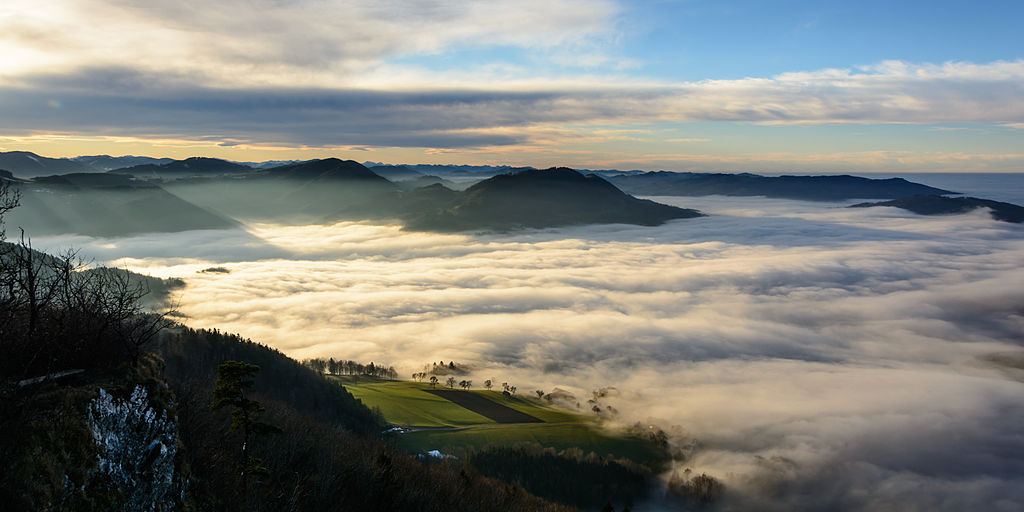
\includegraphics[width=\textwidth]{images/valley.jpg}\end{center}}

\section*{Conclusion}

\begin{frame}{Summary}

  Get the source of this theme and the demo presentation from

  \begin{center}\url{github.com/matze/mtheme}\end{center}

  The theme \emph{itself} is licensed under a
  \href{http://creativecommons.org/licenses/by-sa/4.0/}{Creative Commons
  Attribution-ShareAlike 4.0 International License}.

  \begin{center}\ccbysa\end{center}

\end{frame}

\plain{}{Questions?}

\end{document}
